\documentclass{llncs}

\usepackage{hyperref}
\hypersetup{
    colorlinks,
    citecolor=black,
    filecolor=black,
    linkcolor=black,
    urlcolor=black
}
\usepackage{makeidx}  
\usepackage{amsmath}
\usepackage{amsfonts}
\usepackage{amssymb}
\usepackage{listings}
\usepackage{graphicx}
\usepackage[rightcaption]{sidecap}
\setcounter{tocdepth}{2}
\usepackage{hyperref}
\usepackage{pythonhighlight}

\begin{document}

         % for the preliminaries
%
\title{Diseño, implementación, evaluación y añálisis de un Sistem de Recuperación de Información}
\author{David Orlando De Quesada Oliva, Javier Dom\'inguez}
\institute{MATCOM, Universidad de La Habana.\\
\email{d.quesada@estudiantes.matcom.uh.cu, j.dominguez@estudiantes.matcom.uh.cu}\\
\texttt{}
}
\maketitle

\begin{abstract}
    
    Este art\'iculo aborda sobre la implementación de un Sistema de Recuperación de Información usando 
    el modelo vectorial y el modelo fuzzy para la recuperación de documentos de texto de diversos 
    formatos.

   \keywords{pdf, txt, idf, tf, peso, nltk, fuzzy, vectorial}
\end{abstract}

\tableofcontents
%

% start of the contributions

\chapter*{Dise\~no}
\addcontentsline{toc}{chapter}{Dise\~no}
El sistema está diseñado, primero que todo, para pre-procesar los documentos que están en este.
Este pre-procesamiento consiste en: \\

\noindent $\bullet$ Remover los stopwords (preposiciones, conjunciones y artículos). \\
$\bullet$ Remover los signos de puntuación.\\
$\bullet$ Remover los números.\\
$\bullet$ Llevar todas las palabras a minúscula.\\
$\bullet$ Stemming (llevar cada palabra a su palabra raíz).\\
$\bullet$ Separar por palabras el documento (tokenizar).\\

Los primeros 4 procesos en la implementación son modficables, o sea, es posible decidir si aplicarlos o no.\\

\chapter*{Herramientas usadas para el el desarrollo del sistema}
\addcontentsline{toc}{chapter}{Herramientas usadas para el el desarrollo del sistema}

Para el desarrollo del sistema usamos Python como lenguaje de programación. Librerías de Python
que utilizamos:\\

\noindent $\bullet$ nltk, para los stopwords, stemming y lemmatizing. \\
$\bullet$ streamlit para la interfaz gráfica. \\
$\bullet$ pdfminer y fpdf para procesar archivos .pdf.\\

Para correr la aplicación: {\bf streamlit run main.py} \\

Luego del pre-procesamiento es posible realizar las querys al sistema mediante la interfaz gráfica de dos formas,
mediante texto, o mediante otro documento como se muestra en las imágenes siguientes:

\begin{figure}[h]
    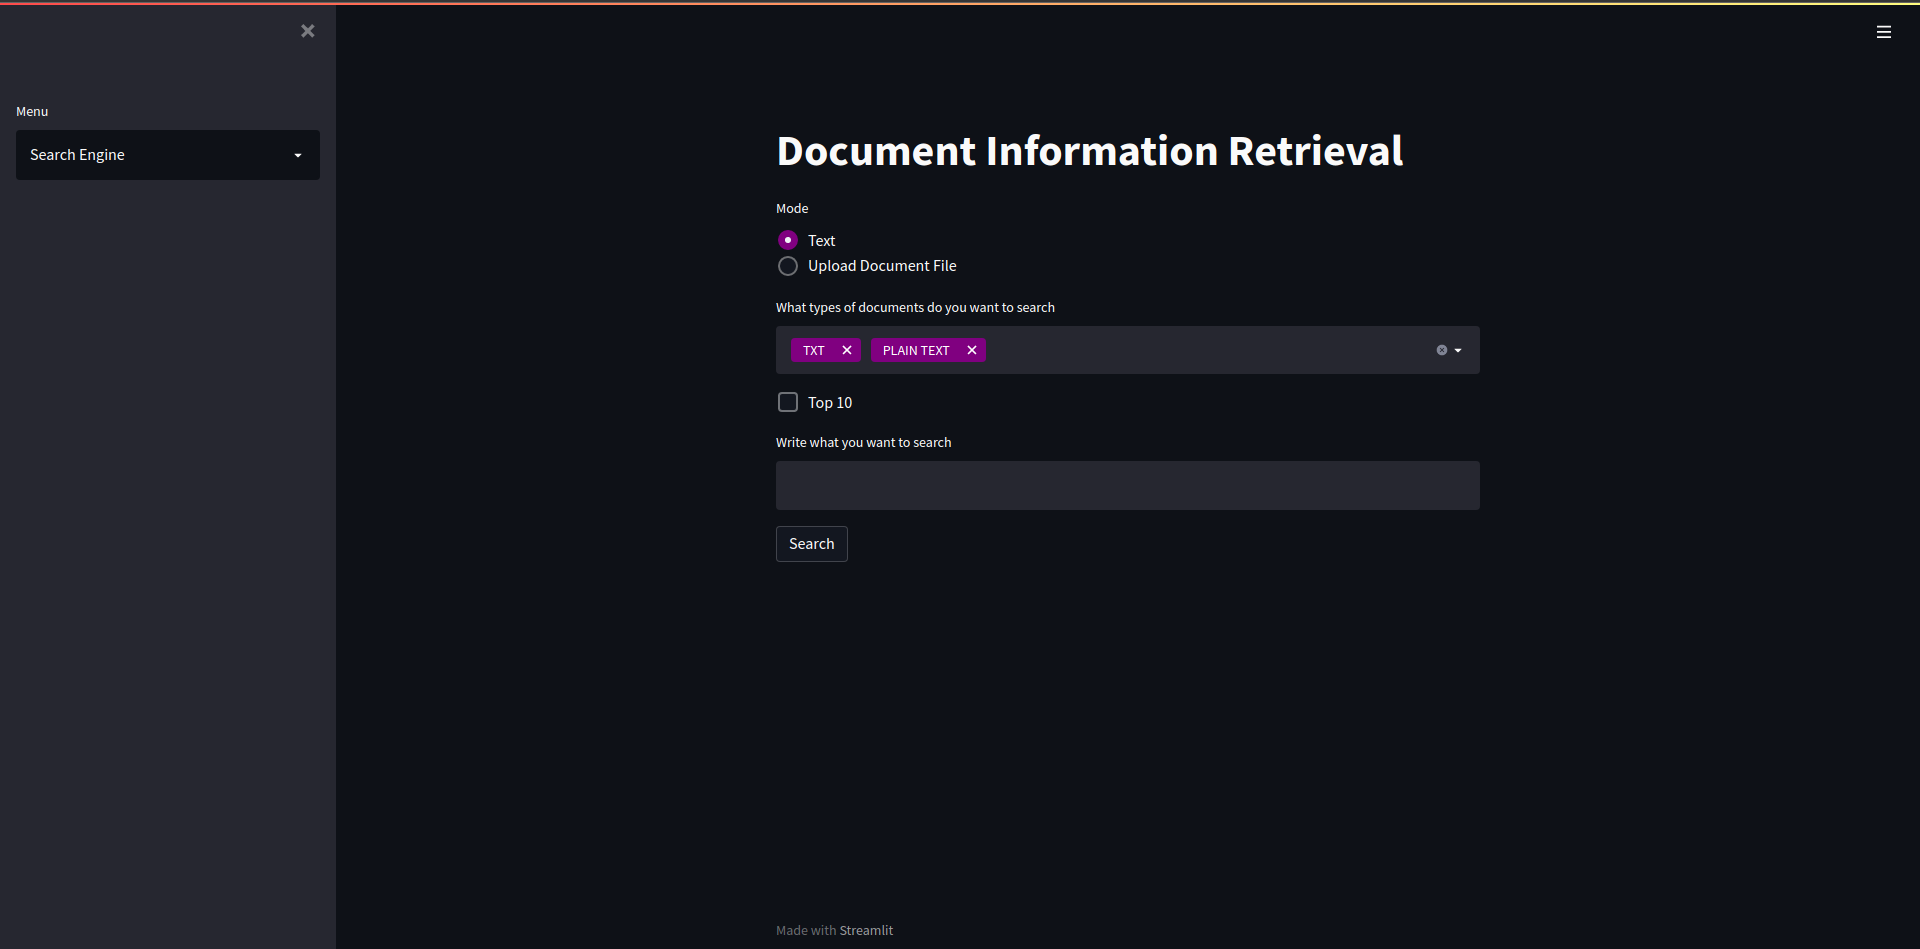
\includegraphics[scale = 0.3]{images/main_screen.png}
\end{figure}

\begin{figure}[h]
    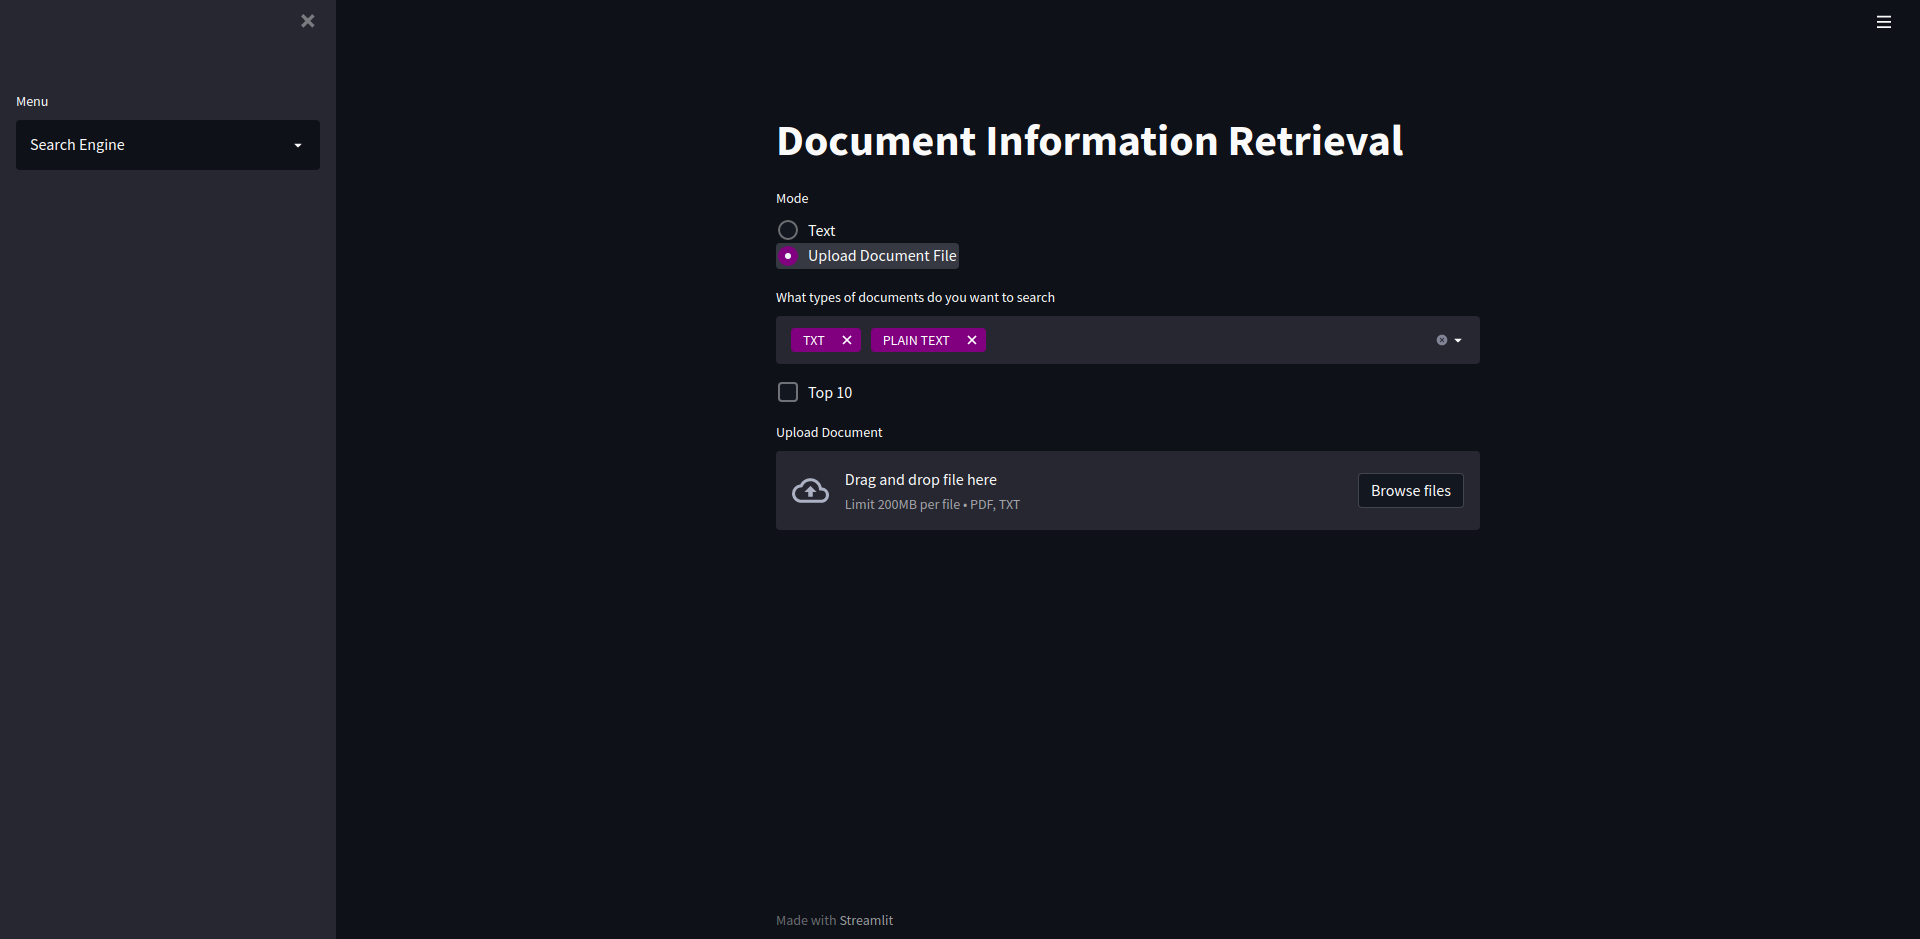
\includegraphics[scale = 0.3]{images/main_upload_file.png}
\end{figure}

\newpage
Es posible escoger que formato de documento es el que se desea buscar:

\begin{figure}[h]
    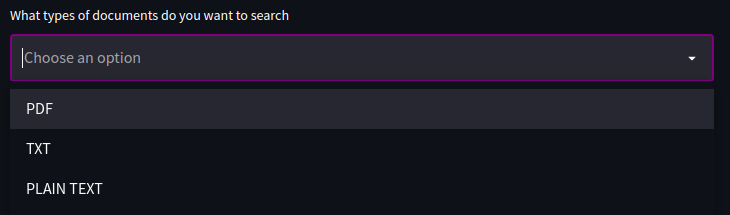
\includegraphics[scale = 0.8]{images/doc_format.png}
\end{figure}

Es posible escoger solamente los 10 elementos más relevantes de la query:\\


\includegraphics[scale = 0.7]{images/top_10.png}

% \newpage
\chapter*{Proceso para la creación de un sistema de recuperación de información}
\addcontentsline{toc}{chapter}{Proceso para la creación de un sistema de recuperación de información}

\section{Preprocesamiento del texto:}

Siempre que tengamos datos textuales, debemos aplicar varios pasos de preprocesamiento a los 
datos para transformar palabras en tokens que permitan un mejor resultado del modelo.
En el sistema de recuperación de información que se implementó es posible aplicar 
los siguientes pasos de preprocesamiento del texto. La implementación de los mismo está en 
el file \textbf{text processing.py}. En muchos pasos hacemos uso de la librería NLTK (Natural Language Toolkit)
de Python.
\\

\noindent
\textbf{Llevar el texto a minúsculas:}
Se lleva todo el texto a minúsculas para reducir el tama\~{n}o del vocabulario de nuestro texto.

\noindent
\textbf{Implementación hecha en Python:}
\begin{python}
    def text_to_lowercase(text: str):
        return text.lower()
\end{python}

\noindent
\textbf{Remover números:}\\
Podemos remover los números o convertir los números en sus representaciones textuales. 

\noindent
\textbf{Implementación hecha en Python haciendo uso de expresiones regulares para eliminar los números:}
\begin{python}
    import re
    def remove_numbers(text):
        return re.sub(r'\d+', '', text)
\end{python}

\noindent
\textbf{Implementación hecha en Python parar convertir los números a sus expresiones textuales haciendo uso de la libería inflect:}
\begin{python}
    import inflect
    def convert_numbers_into_words(text: str)-> str:
        result = []
        for word in text.split(): 
            if word.isdigit(): 
                result.append((inflect_engine.number_to_words(word)))
            else:
                result.append(word)

        return ' '.join(result)
\end{python}


\noindent
\textbf{Remover los signos de puntuación:}\\ 
\noindent
Eliminamos los signos de puntuación para no tener diferentes formas de la misma palabra. 
Si no eliminamos los signos de puntuación, entonces  por ejemplo \textbf{call.} \textbf{call!} 
\textbf{,call}  serán tratados por separado cuando deberían referirse a la misma palabra.
\\
\textbf{Implementación hecha en Python parar remover los signos de puntuación:}
\begin{python}
    def remove_punctuation_marks(text: str):
        translator = str.maketrans('', '', string.punctuation)
        return text.translate(translator)
\end{python}

\noindent
\textbf{Remover los stopwords:}\\ 
\noindent
Los stopwords son palabras que no contribuyen al significado de una oración. Por tanto
pueden eliminarse con seguridad sin causar algún cambio en el significado de la oración.
La biblioteca NLTK tiene un conjunto de stopwords y podemos usarlas para eliminar 
los stopwords de nuestro texto y devolver una lista de tokens de palabras. 

\begin{SCfigure}[0.6]
    \caption{Lista de stopwords de NLTK}
    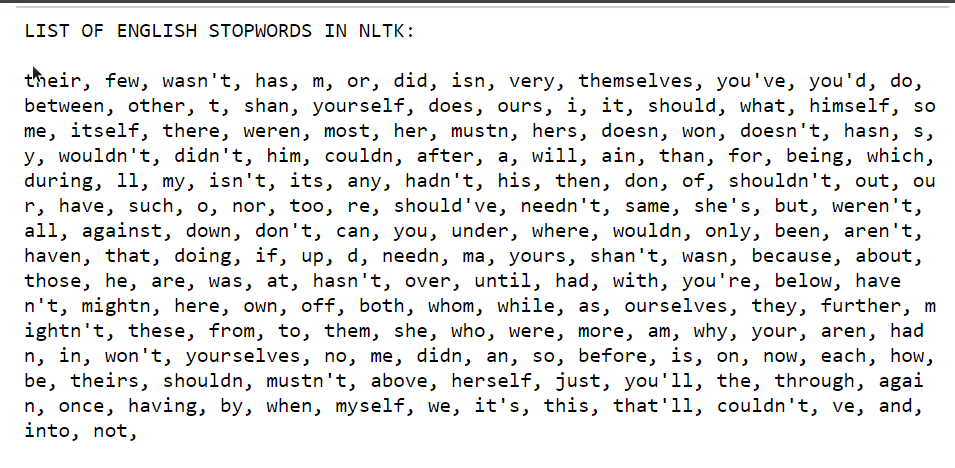
\includegraphics[scale = .3]{./images/englis_stopwords_nltk.png}
\end{SCfigure}

\noindent
\textbf{Implementación hecha en Python para el proceso de eliminar los stopwords}

\begin{python}
    from nltk.corpus import stopwords
    def text_remove_stopword(text: str):
        stop_words = set(stopwords.words("english"))  
        return ' '.join([word for word in text_tokenize(text) if word not in stop_words])
    
\end{python}

\noindent
\textbf{Stemming:}\\ 
\noindent
El stemming es el proceso mediante el cual se obtiene la raíz gramatical de una palabra. 
Stem es la parte a la que se le añaden los afijos flexivos (-ed, -ize, -de, -s, etc. En el caso del idioma inglés)
El stem de una palabra es creado removiendo el prefijo o sufijo de la palabra. Por lo que el proceso
de stemming de una palabra puede no resultar en palabras gramaticalmentes correctas del idioma

\begin{SCfigure}[0.6]
    
    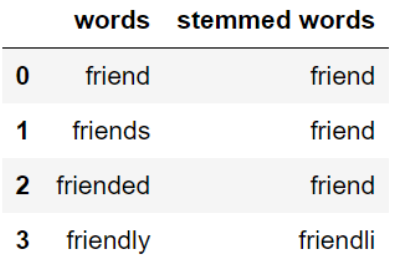
\includegraphics[scale = .3]{./images/stemming1png.png}
    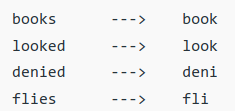
\includegraphics[scale = .7]{./images/stemming2png.png}
    \caption{Ejemplos del proceso de stemming en algunas palabras}
\end{SCfigure}

Hay principalmente 3 algoritmos para hacer stemming \textbf{Porter Stemming}, 
\textbf{ Snowball Stemmer} y el \textbf{Lancaster Stemmer}. El Porter Stemming 
es el más usado entre ellos.
\\\\
\textbf{Implementación hecha en Python para hacer el proceso de stemming. Se puede pasar como parámetro un string que indica con cual de los tres algoritmos se quiere hacer stemming.}

\begin{python}
    from nltk.stem.porter import PorterStemmer
    from nltk.stem.snowball import SnowballStemmer
    from nltk.stem.lancaster import LancasterStemmer

    porter_stemmer =  PorterStemmer()
    snowball_stemmer = SnowballStemmer(language='english')
    lancaster_stemmer = LancasterStemmer()
\end{python}


\begin{python}
    def text_stem_words(text: str, stemmer: str):
        if text == 'porter':
            stemmer = porter_stemmer
        elif text == 'snowball':
            stemmer = snowball_stemmer
        else:
            stemmer = lancaster_stemmer

        stems = [stemmer.stem(word) for word in text_tokenize(text)]
        return ' '.join(stems)
\end{python}

\noindent
\textbf{Lemmatizing:}\\
Como el stemming, el proceso de lemmatizing también convierte una palabra
a su raíz gramatical. La única diferencia es que el lemmatizing asegura que
la raíz gramatical de la palabra pertenezca al lenguaje. Obtenemos palabras
válidas si usamos el lemmatizing. En \textbf{NLTK}, podemos hacer uso del 
\textbf{WordNetLemmatizer} para obtener los lemmas de las palabras. 

\noindent
\textbf{Implementación en Python para el proceso de lemmatizing usando el WordNet de NLTK}

\begin{python}
from nltk.stem import WordNetLemmatizer
lemmatizer = WordNetLemmatizer()
def text_lemmatize_words(text: str):
lemmas = [lemmatizer.lemmatize(word, pos ='v') for word in text_tokenize(text)]
return ' '.join(lemmas)
\end{python}

\noindent
\textbf{Separar el texto en tokens:}\\
El último paso que hacemos siempre (este paso es necesario) 
es separar el texto en una lista de tokens de palabras 
removiendo los espacios. Para eso hacemos uso del word tokenize 
de NLTK.
\\\\
\noindent
\textbf{Implementación en Python para separar el texto en tokens}

\begin{python}
from nltk.tokenize import word_tokenize
def text_tokenize(text: str):
    tokens = word_tokenize(text)
    return tokens
\end{python}
\noindent
De la forma en que está hecho el código se le puede pasar uno o varios pasos de preprocesamiento 
al texto según se requiera. 
\\
\begin{python}
def text_preprocessing(*, text: str, 
    lowercase: bool = False, 
    remove_numbers: bool = False,
    convert_numbers: bool = False,
    remove_punctuation: bool = False,
    stopwords: bool = False,
    stem: str = None,
    lemmatize: bool = False):
    ...
\end{python}
El método recibe un texto y se le pasan en True los parámetros con los que
se quiere filtrar el mismo. En el caso del parámetro stem se le pasa un string 
que indica con cual de los algoritmos se va a hacer el stemming. 

\noindent
\textbf{Configuración predeterminada empleada:}
\begin{python}
def filter_and_tokenize_text(text: str):
    tokens = text_preprocessing(
                text=text,
                lowercase = True,
                convert_numbers= True,
                remove_punctuation=True,
                stopwords=True,
                lemmatize=True

            )

    return tokens
\end{python}

\noindent
Este preprocesado de texto se le hace tanto a los documentos en el sistema como
a cada query que se procese del usuario.

\section{Tokenización de los documentos del sistema y creación del vocabulario de las palabras:}
Por defecto todos los documentos que tiene el sistem están en el path:
\begin{python}
'.\system_docs'
\end{python}

Para el preprocesado de los documentos del sistema se va por cada file del path y
se lee el texto del documento(la forma de leer varía según el formto del mismo, consideramos
aceptar .txt, pdfs y textos planos sin extensión) contruimos una instancia de Doc con el nombre 
del documento, el path donde está realmente(útil para cuando el usuario haga la búsqueda
pueda descargar el documento original), el tipo (TXT, PDF, o Texto Plano son los que consideramos),
y el texto que al inicializarse se procesa el texto como se explicó  previamente y nos quedamos con una lista 
de tokens que representan las palabras que tienen significación en ese el texto.
\begin{python}
class Doc:

    def __init__(self, name: str, path: str, type: str, text= str):
        self.name = name
        self.path = path
        self.type = type
        self.terms = filter_and_tokenize_text(text)
    ...
\end{python}

Si en el path hay un folder se va recursivo por cada folder y se aplica lo mismo. De esta forma se va
construyendo una lista de Doc que representan la información necesaria de los documemntos que hay en el 
sistema. Al mismo tiempo se construye una lista con todos los términos distintos que aparecen en todos 
los documentos. Hacer estas operaciones son bastante costosas cuando se tienen bastante documentos en 
el sismtema por lo que se hace solo cuando sea necesario porque se cambió o añadió nuevos documentos.
Por lo que una vez obtenido las dos listas se serializa y guarda con \textbf{pickle} en los files 
{documentos.pickel} y \textbf{terms.pickle}. De esta forma no hay que estar generando cada vez sino que
se lee el archivo.

El código de implementación de este proceso está en 
\begin{python}
    system_docs_preprocessing.py
\end{python}

Para decir que se quiere hacer el preprocesado de los documentos del sistema y generar nuevos files 
se llama al handler con el parámetro system docs preprocess required en True
\begin{python}
handler =  Retrieval_handler(system_docs_preprocess_required=True,
     model_preprocess_required=True, retrieval_model_used='vectorial')
    ...
\end{python}

En caso que sea False el handler internamente cargará los files pickle correspondientes.


\section{Modelo vectorial:}
El modelo principal que usamos para el sistema de recuperación de información fue el vectorial.
Este modelo representa los documentos como vectores en un espacio vectorial común, donde cada 
dimensión corresponde a un término independiente. \\
Por ejemplo: \\
Sea dj el documento j y i,...t el t-ésimo término entonces el vector del documento j quedaría:\\
$
    d_j = (w_{1,j}, w_{2,j}, ..., w_{t,j})
$

\noindent
Si aparece un término en el documento, su valor 
en el vector es distinto de 0. El esquema usado para calcular estos valores se conoce como
\textbf{tf-idf weighting}. El peso(weight) asociado al par $(t_i, d_j)$ es $>=0$. 
\\\\
\noindent
\textbf{Calculo del peso en los documentos:}\\\\
\noindent
El peso del término \textbf{$t_i$} en el documento $d_j$ está dado por:\\
\\
$
    w_{i,j} = tf_{i,j}* idf_i
$
\\\\
El \textbf{idf(inverse document frequency)} de un término i se define:\\
\\
$
    idf_i = log{\frac{N}{n_i}}
$
\\\\
Donde N es la cantidad de documentos existentes en el sistem y $n_i$ la cantidad 
de documentos en los que aparece el término $t_i$.
\\\\
La frecuencia normalizada del término $t_i$ en el documento $d_j$ se define como:
\noindent\\\\
$
    t_{i,j} = \frac{freq_{i,j}}{max_lfreq{l,j}}
$
\\\\
Donde $freq_{i,j}$ es la frecuencia del término $t_i$ en el documento $d_j$ y
$max_lfreq{l,j}$ la máxima frecuencia que tiene un término l en el documento j.
\\\\
\noindent
\textbf{Para representar este modelo creamos una clase Vectorial} 
\\
\begin{python}
def __init__(self, corpus_term, documents, compute_vectorial_data_required: bool = False):
    self.a = 0.4 # suavizado
    self.corpus_terms = corpus_term # list to store the terms present in the documents
    self.documents = documents # documents of the corpus of the form Doc()
    if compute_vectorial_data_required:
        self.compute_docs_vectors()
    else:
        self.d_vectors = unpick_pickle_file('./preprocessed/d_vectors.pickle')
        self.idf = unpick_pickle_file('./preprocessed/idf.pickle')
    ...
\end{python}
\noindent
la cual se inicializa con el vocabulario y la lista que tiene la representación
de cada documento del corpus asi como con un parámetro opcional que indica que es necesario
calcular el vector de cada documento o se lee directo de un file .pickle serializado, 
esto es debido a que hacer este proceso es extremadamente costoso por lo que se hace previamente
y solo es necesario volverlo a cambiar si cambia el corpus(se agregan o modifican nuevos documentos).
\\
Con el método:
\begin{python}
    def compute_docs_vectors(self):
    ...
\end{python}
\noindent
se calculan el vector de cada documento con el esquema idf-tf para calcular los pesos de
cada documento con cada término del vocabulario del corpus.

\begin{python}
    N = len(self.documents)
    len_terms = len(self.corpus_terms)
    d_vectors = [ len_terms*[0] for _ in range(N) ]
    tf = [N*[0] for _ in range(len_terms)]
    idf = len_terms*[0]
    for doc_id,doc in enumerate(self.documents):

    if doc.terms: 
        freq_counter = Counter(doc.terms)
        max_freq_dj  = freq_counter.most_common(1)[0][1] 
        for term_id, term in enumerate(self.corpus_terms):
            freqij = freq_counter[term]
            tf[term_id][doc_id] = freqij/max_freq_dj 
    ...
\end{python}

\noindent
Primero se computa el tf para cada término del corpus con cada documento y se guarda 
en una lista tf tal que $tf[t_i][d_j]$ me de el tf del término con posición $t_i$ en la lista
de términos y del documento con posición $d_j$ en la lista de documentos.
\\\\
\begin{python}
    terms_appear = len_terms*[0] 
        for term_id, term in enumerate(self.corpus_terms):
            for doc in self.documents: 
                if term in doc.terms:
                    terms_appear[term_id]+=1
    ...
\end{python}

Luego calculamos para cada término la cantidad de documentos en los que este aparece y lo guardamos 
en la lista $terms_appear$
\\\\
\begin{python}
    for term_id,term in enumerate(self.corpus_terms):
        idf[term_id] =  math.log(N/terms_appear[term_id])
    ...
\end{python}

Luego se calcula el idf para cada término usando la lista previamente calculada $terms_appear$ para obtener 
el $n_i$ de cada término y guardamos el resultado en la lista idf.
\\\\
\begin{python}
    for dj in range(N):
            for term_id, _ in enumerate(self.corpus_terms):
                d_vectors[dj][term_id] = tf[term_id][dj] * idf[term_id]
    ...
\end{python}
\noindent
Luego vamos por cada documento $d_j$ y cada término $t_i$ y se calcula el peso $w_{i,j}$ 
usando las listas de tf e idf previamente calculadas y finalmente nos queda un vector 
de cantidad de términos en el vocabulario componentes por cada documento del corpus. 
\\\\
Finalmente se serializan la lista de vectores y el idf(necesario para calcular el peso de las query)
usando pickle y se guarda en los files $d\_vectors.pickle$ y $idf.pickle$
\\\\
\noindent
\textbf{Querys en el modelo vectorial}:\\\\
Las querys también se representan como un vector q\\
\noindent
$
    q =(w_{1,q}, w_{2,q},...,w_{n,q})
$
\noindent
\\
El cálculo del peso es bastate similar a como es con los documentos 
con la diferencia que se introduce una constante de suavizado a.
\\\\
$
    w_{i,q} = (a+(1-a)*\frac{freq_{i,q}}{maxlfreq_{l,q}})
$

\begin{python}
    def compute_query_vector(self, query: str):
    ...
\end{python}

con este método se computa el vector de una query.

Luego de hacer primero el preprocesado del texto y terner los tokens
calculamos el peso como se ve a contincuación:
\begin{python}
    q_vector = len(self.corpus_terms)*[0]
    if tokens:
        freq_counter = Counter(tokens)
        max_freq_q  = freq_counter.most_common(1)[0][1] 
        for ti, term in enumerate(self.corpus_terms):
            freqiq = freq_counter[term] 
            tf_ti_q = self.a + (1 - self.a)* (freqiq/max_freq_q) 
            idf_ti = self.idf[ti] 
            w_iq = tf_ti_q * idf_ti 
            q_vector[ti] = w_iq
    return q_vector
    ...
\end{python}

La query puede ser vacía(no tener ningún término) en dicho caso el vector sería 0 en cada una de sus componentes.
\noindent
\textbf{Cálculo de la similitud:}\\
El cálculo de similitud entre un documento y la query se hace comparando la desviación de ángulos entre el vector del documento 
y el vector de la query(la cual tiene dimensión igual a los vectores que representan los otros documentos).
\\\\

\begin{SCfigure}[0.6]
    \caption{Visualización con vectores de 2 dimensiones}
    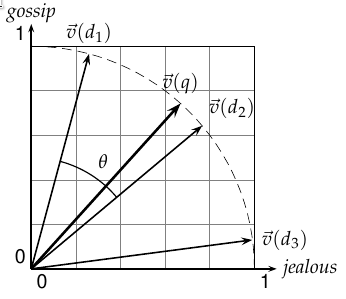
\includegraphics[scale = .5]{./images/ejemplosim.png}
\end{SCfigure}

Para calcular la similitud hacemos
$
    sim_{d_j, q} = cos{\theta}=\frac{d_j*q}{||d_j||||q||} = \frac{\sum_{n = 1}^{N} w_{i,j}w_{i,q} }
    { \sqrt{\sum_{n = 1}^{N} w_{i,j}^{2} } \sqrt{\sum_{n = 1}^{N} w_{i,q}^{2} }}
$

Con esto se tiene una ordenación por relevancia(los que tengan mayor similitud) de 
de los documentos respecto a la query .

\textbf{Implementación realizada en Python para el cálculo de la similitud}

\begin{python}
    def sim(self, v1: List[float], v2: List[float]) -> float:
        dotproduct = 0
        for i in range(len(v1)):
            dotproduct += v1[i]*v2[i]

        norm1 = 0
        for i in v1:
            norm1 += i*i
        norm1 = math.sqrt(norm1)

        norm2 = 0
        for i in v2:
            norm2 += i*i
        norm2 = math.sqrt(norm2)

        return dotproduct/(norm1*norm2)
    ....
\end{python}


Se puede establecer un umbral de similitud y quedarnos solamente con los documentos que son mayores 
que ese umbral.

\subsection {Razones por la que se escogió este modelo como el modelo principal del sistema:}
\noindent
$\bullet$
Este modelo es bastante sencillo de implementar y ofrece notables mejoras respecto al booleano.\\
\noindent
$\bullet$
La estrategia de coincidencia parcial permite la recuperación de documentos que se aproximen a los 
requerimientos de la consulta. \\
\noindent
$\bullet$
El esquema de ponderación tf-idf para los documentos mejora el 
rendimiento de la recuperación. \\
\noindent
$\bullet$
La fórmula del coseno ordena los documentos 
de acuerdo al grado de similitud con la consulta. 

\subsection {Limitaciones que tenemos al usar este modelo:}
$\bullet$
Uno de los problemas que tiene es la sensibilidad semántica; los documentos con un contexto similar 
pero con un vocabulario de términos diferente no se asociarán, lo que resultará en una coincidencia 
negativa falsa.\\
\noindent
$\bullet$
Teoricamente asume que los términos son estáticamente independientes\\
\noindent
$\bullet$
El orden en que los términos aparecen en el documento se pierde en la representación en el espacio vectorial

\section{Modelo Fuzzy:}
Se implementó como modelo secundario para tener la opción de elegir si se quería probar con el mismo. 

El modelo fuzzy es una extensión del modelo booleano. En este modelo cada término de la query es 
definido mediante un conjunto difuso y cada documento tiene un grado de pertenencia a dicho 
conjunto(valor entre 0 y 1). La idea básica es expandir el conjunto de términos de índice 
en la consulta con términos relacionados, de modo que la consulta del usuario pueda recuperar 
documentos relevantes adicionales. Se puede usar un thesaurus para modelar el problema de recuperación 
de información en términos de conjuntos difusos. Un thesaurus puede ser construido definiendo una 
matriz de correlación término a término cuyas filas y columnas están asociada a los términos  de la
colección de documentos. En dicha matriz, un factor de correlación normalizado $c_{i,l}$ entre 
dos términos $k_{i}$ y $k_{l}$ se define de la siguiente forma:\\

$
    c_{i,l} =  \frac{n_{i,l}}{n_i+n_l-n_{i,l}}
$
\\\\
\noindent
Donde $n_i$ es el número de documentos que contienen al término $k_i$, $n_l$ el número de documentos
que continen al término $k_l$, $n_{i,l}$ el  número de documentos que contienen a ambos términos \\
Podemos usar la matriz de correlación para definir un conjunto difuso asociado a cada término $k_i$.
En este conjunto difuso, un documento $d_j$ tiene un grado de pertenencia(grade of membership) $\mu_{i,j}$
que se define como:\\\\
$
\mu_{i,j} = 1 - \prod_{k_ln \in d_j}^{}  (1-c_{i,l}) 
$
\\\\
\noindent
Un documento $d_j$ pertenece al conjunto difuso asociado al término $k_i$ si sus  términos están relacionados 
con $k_i$. Siempre que haya un término $k_l$ de $d_j$ que esté fuertemente relacionado($c_{i,l}\sim 1$), 
entonces $\mu_{i,j} \sim 1$ y el término $k_i$ es un buen fuzzy index para el documento $d_j$. En el caso 
que todos los documemntos de $d_j$ estén pobremente relacionados con $k_i$, $k_i$ no es un buen fuzzy 
index para $d_j$($\mu_{i,j}\sim 0 $).\\\\ 

La similitud entre un documento $d_j$ y la query q se se define:

$
    sim(q,d_j) = 1 - \prod_{i=1}^{N} (1 - \mu_{k_i,d_j})
$

Donde N es la cantidad de términos de la query.

Entonces te puedes quedar con los documentos ordenados por ranking de relevancia 
respecto a la query.

Para la implementación de este modelo se definió una clase Fuzzy
\begin{python}
class Fuzzy:
def __init__(self, corpus_term, documents, compute_fuzzy_data_required: bool = False):
    self.corpus_terms: List['str'] = corpus_term 
    self.documents: List['Doc'] = documents
    self.correlation_matrix = {}
    if compute_fuzzy_data_required:
        self.compute_fuzzy_data()
    else:
        self.deg_memb_matrix = unpick_pickle_file('./preprocessed/deg_memb_matrix.pickle')
    ...
\end{python}

Recibe los términos del vocabulario y los documentos asi como el parámetro $compute\_fuzzy\_data\_required$
que indic si es necesario hacer el preprocesado de calcular la matriz de grado pertenencia o se 
puede cargar desde un file previamente salvado \textbf{.pickle}\\\\
\noindent
\textbf{Implementación hecha en Python para el c\'alculo de la matriz de correlación:}
\begin{python}
def correlation_factor(self, ki: str, kl: str):
    if (ki,kl) in self.correlation_matrix:
        return self.correlation_matrix[(ki, kl)]
    if (kl, ki) in self.correlation_matrix:
        return self.correlation_matrix[(kl, ki)]
    n_i = 0  
    n_l = 0
    n_i_l = 0 
    for doc in self.documents:
        if ki in doc.terms:
            n_i+=1
        if kl in doc.terms:
            n_l+=1
        if ki in doc.terms and kl in doc.terms:
            n_i_l +=1
    result = n_i_l/(n_i + n_l - n_i_l) # ci,l
    self.correlation_matrix[(ki, kl)] = result
    return result
...
\end{python}
\textbf{Implementación hecha en Python para el c\'alculo del grado de pertenencia 
de un documento dj al conjunto difuso de un término ki:}\\
\begin{python}
    def degree_of_membership(self, ki, dj): 
        if (ki, dj) in self.deg_memb_matrix:
            return self.deg_memb_matrix[(ki, dj)]
        result = 1
        for term in self.documents[dj].terms:
            result *= 1- self.correlation_factor(ki, term)
        result = 1 - result
        return result
    ...
\end{python}

\noindent
\textbf{Implementación hecha en Python para el cálculo de la similitud 
entre la query y un documento:}\\

\begin{python}
    def sim(self, q, dj): 
        result = 1

        for t in q:
            result *= 1 - self.deg_memb_matrix[(t, dj)]

        result = 1- result
        return result
    ...
\end{python}


Para obtener los documentos más relevantes se va por cada documento se calcula 
la similitud de cada uno con la query como se explicó anteriormente y al 
final se hace un ranking por relevancia bastante similar a como es con el vectorial.
También se puede considerar un umbral de similitud y quedarte solamente con los resultados
por encima de dicho umbral.

\section{Evaluación del Modelo Vectorial:}


\section{Interfaz gráfica y como puede buscar las consultas el usuario:}

La interfaz gráfica se desarrollócon \textbf{streamlit} una biblioteca bastante cómoda para 
crear aplicaciones de interfaz web desde Python. En el file $UI\_streamlit.py$ 
está el código de la parte gráfico del sistema de recuperación de información 
desarrollado.




% El campo de la recuperación de imágenes ha demostrado ser uno necesario para los tiempos en que vivimos, donde tantas imágenes 
% se generan diariamente, desde satélites orbitando la Tierra, misiones espaciales en lo más lejos del cosmos, 
% animales en la naturaleza, paisajes, cámaras de seguridad y mucho más. Las imágenes son una fuente de información 
% muy útil en la actualidad, y por tanto almacenarlas y organizarlas es una tarea necesaria, para facilitar 
% el acceso a la información. De ahí que este campo tenga una gran cantidad de aplicaciones en la actualidad, 
% a continuación mencionamos algunas de las más importantes:
% \\\\
% \noindent $\blacksquare$ \textbf{El problema de la anotación automática de imágenes.}\\
% El propósito principal de un sistema de recuperación de imágenes basado en contenido es descubrir imágenes que pertenecen a algún 
% concepto, en la ausencia de meta-datos, todos los intentos de automatizar el proceso de creación de estos meta-datos tiene ese 
% objetivo. La anotación de imágenes puede facilitar la búsqueda de imágenes utilizando texto. Si el mapeo resultante imagen-palabras 
% clave es confiable, la búsqueda de imagen basada en texto puede tener semánticamente más sentido que buscar en la ausencia de texto. 
% Uno de los métodos para resolver este problema de la anotación automática es usar aprendizaje supervisado para categorizar las 
% imágenes. La detección de conceptos simples como: paisaje, ciudad, animales, etc, alcanza una alta precisión.
% \\\\
% \noindent $\blacksquare$El arte y la cultura siempre han sido importantes en la vida del ser humano. A lo largo de la historia, los museos y galerías 
% de arte del mundo se han encargado de preservar nuestra diversa herencia cultural para utilizarlos como fuentes educación y 
% aprendizaje. Es por esto que recientemente se ha expresado la preocupación por digitalizar todos los materiales antiguos, 
% históricos y culturales, para la posteridad. Esto es muy importante por dos razones, primero las computadoras se han convertido 
% en el principal medio de aprendizaje y se supone que así sea durante los próximos años, por tanto la representación digital de 
% los artefactos culturales y las imágenes es algo que facilitará su popularidad, además de que sería accesible desde cualquier 
% rincón del mundo, y segundo al contrario de la información almacenada de forma digital, los artefactos y pinturas antiguas están a 
% merced a la degradación con el paso del tiempo, a los desastres y al vandalismo.
% \\\\
% \noindent $\blacksquare$ Las interacciones entre CBIR y la seguridad de la información ha sido prácticamente nulo, hasta que recientemente ciertas perspectivas 
% han emergido  para unir ambos campos, las pruebas de interacción humana (HIPs por sus siglas en inglés) y el cumplimiento de 
% la protección de los derechos de autor. Mientras por un lado constantemente estamos ampliando las fronteras de la ciencia para 
% diseñar sistemas que pueda imitar las capacidades humanas, no podemos negar los riesgos de seguridad inherentes asociados con 
% programas extremadamente "inteligentes". Uno de dichos riesgos es cuando un sitio web o algún servidor es atacado por programas 
% maliciosos que solicitan servicios a escalas masivas. Pueden ser escritos programas que consuman una gran cantidad de recursos web o 
% que influyan en los resultados de votaciones. En este caso los HIPs también conocidos como CAPTCHAs, son la solución. Estas interfaces 
% están diseñadas para diferenciar entre humanos o programas, basados en la respuesta a algunas preguntas.

% \noindent $\blacksquare$ \textbf{Aplicaciones en la medicina} :
% Una apliaci\'on que recupera cortes de 2D MRI(im\'agenes de resonancia magn\'etica)
% de vol\'umenes cerebrales en 3D. La aplicaci\'on aceptar\'ia query de im\'agenens 2D MRI del usuario e identificar\'ia el volumen 3D que coincide
% de acuerdo con la  regi\'on del cerebro relacionada con la query. Los cortes coincidentes se recuperadan mediante una b\'usqueda adicional en los vol\'umenes
% 3D coincidentes.

% \noindent $\blacksquare$ \textbf{Aplicaciones en el comercio electr\'onico} :
% La compra electr\'onica es la tendencia actual en el mundo m\'as que compras tradicionales debido a la conveniencia de internet. Cuando llega 
% el tiempo de la compra, los usuarios se encuentran con un problema en seleccionar los items que necesitan comprar. Un sistema de recuperaci\'on
% de im\'agenes puede asistir a la decisiones del usuario en ropa y ayudarlo a tener una mejor selecci\'on de ropa durante la compra electr\'onica.
% El m\'etodo usado enriquece la b\'usqueda y recuperaci\'on de productos de informaci\'on usando CBIR con caracter\'isticas como el color o la textura 
% en la aplicaci\'on de la venta minorista de ropa electr\'onica.  

% % \newpage

% \chapter*{Ventajas y desventajas}
% \addcontentsline{toc}{chapter}{Ventajas y desventajas}

% \underline {\bf Keyword Based Image Retrieval}\\

% Ventajas:\\
% \noindent$\bullet$ La realizaci\'on de queries mediante texto suele ser m\'as intuitiva y f\'acil para los usuarios.\\

% Desventajas:\\
% \noindent$\bullet$ No tiene en cuenta conceptos sem\'anticos.\\
% $\bullet$ Solo usando texto para describir el contenido de una imagen a menudo causa ambig\"{u}edad e insuficiencia en el rendimiento
% de la b\'usqueda de im\'agenes en una base de datos y el procesamiento de las queries de los usuarios.\\

% \underline {\bf Content Based Image Retrieval}\\

% Ventajas:\\
% \noindent$\bullet $ Las queries se pueden realizar utilizando alguna imagen en algunos casos.\\
% $\bullet $ Se computan las caracter\'isticas de bajo nivel para lograr una mayor precisi\'on a la hora de responder a una 
% query.\\

% Desventajas:\\
% \noindent$\bullet$ Los sistemas basados en esta t\'ecnica sufren de lo que se denomina brecha sem\'antica. Es una brecha 
% entre los complejos conceptos sem\'anticos que puede percibir el ser humano, y que las m\'aquinas no son capaces de
% comprender f\'acilmente.\\

% \underline {\bf Semantic Based Image Retrieval}\\\\

% Ventajas:\\
% \noindent$\bullet$ Es capaz de utilizando herramientas de machine learning lograr una mayor precisi\'on a la hora de representar conceptos sem\'anticos.\\

% Desventajas:\\
% $\bullet$ A pesar de que estos sistemas son mucho mejores que los existentes tiempo atr\'as, a\'un no existen mecanismos lo suficientemente potentes.\\

% \underline {\bf Ontology Based Image Retrieval}\\\\

% Ventajas:\\
% \noindent$\bullet$ Usando la representaci\'on ontol\'ogica  de im\'agenes se puede interpretar las ideas de alto nivel de la mente del usuario.



% Desventajas:\\
% $\bullet$
% Si se define una ontolog\'ia compleja el proceso de anotaci\'on tambi\'en ser\'a complejo. El modelo de dominio ontol\'ogico es tan bueno 
% como la mano experta que decide la ontolog\'ia.

\newpage

\chapter*{}
\addcontentsline{toc}{chapter}{References}
\begin{thebibliography}{}
    %
    \bibitem[1]{2clar:eke}
    Ritika Hirwane(2012).
    Fundamental of Content Based ImageRetrieval.
    (IJCSIT) International Journal of Computer Science and Information Technologies, Vol. 3 (1)
    
    \bibitem[2]{2clar:eke:2}
    Hui Hui Wang, Dzulkifli Mohamad, N.A. Ismail(2010).
    Approaches, Challenges and Future Direction
    of Image Retrieval.
    Journal of Computing, Volume 2, Issue 6
    
    \bibitem[3]{2mich:tar}
    Chandra Mouli P.V.S.S.R.,Mohd Khalid
    Vijayan Vijayarajan(2012).
    A review: from keyword based image retrieval to ontology 
    based image retrieval.International Journal of Reviews in Computing  
    
    \bibitem[4]{2tar}
    John Eakins,Margaret Graham(1999).
    Content-based Image Retrieval.
    JISC Technology Applications Programme (October 1999)

    
    \bibitem[5]{2rab}
    Yu Xiaohong, Xu Jinhua(2008)
    The Related Techniques of Content-based Image Retrieval.
    2008 International Symposium on Computer Science and Computational Technology
    
    \bibitem[6]{2rab}
    Elsaeed E. AbdElrazek(2017).
    A Comparative Study of Image Retrieval Algorithms for
    Enhancing a Content-based Image Retrieval System.
    Global Journals  of Computer Science and Technology:Inc Volume 17 Issue 3 Version 1.0

    \bibitem[7]{2rab}
    Abby A. Goodrum(2000).
    Image Information Retrieval: An Overview of Current Research.
    College of Information Science and Technology Drexel University.

    \bibitem[8]{2rab}
    Unknown Author(2021,November 26).
    Image retrieval.Wikipedia.\url{https://en.wikipedia.org/wiki/Image_retrieval}.
    
\end{thebibliography}



\end{document}